\section*{Lezione 6}
\addcontentsline{toc}{section}{Lezione 6}

Cominciamo con un esempio: supponiamo di avere una sorgente caratterizzata da quattro simboli, codificati in questo modo:

\begin{equation*}
s_1 \rightarrow 0
\end{equation*}
\begin{equation*}
s_2 \rightarrow 01
\end{equation*}
\begin{equation*}
s_3 \rightarrow 11
\end{equation*}
\begin{equation*}
s_4 \rightarrow 00
\end{equation*}

A questo punto supponiamo che il ricevente riceva la stringa 0011, qual è la sequenza di codeword che ho ricevuto?
Una soluzione potrebbe essere $s_1, s_1, s_3$, ma anche $s_4, s_3$.
Questa codifica e questa sequenza mette in crisi il ricevitore, ed è uno dei casi da evitare (non univocamente decodificabile).


Tra i codici \textbf{univocamente decodificabili} possiamo distinguere due ulteriori sottocasi:
\begin{itemize}
	\item Istantanei: il ricevente appena finito di ricevere una codeword la decodifica senza ambiguità.
	\item Non istantantei: non vale la regola precedente.
\end{itemize}

Vediamo un esempio di codice univocamente decodificabile \underline{non istantaneo}:

\begin{equation*}
s_1 \rightarrow 0
\end{equation*}
\begin{equation*}
s_2 \rightarrow 01
\end{equation*}
\begin{equation*}
s_3 \rightarrow 011
\end{equation*}
\begin{equation*}
s_4 \rightarrow 111
\end{equation*}

Immaginiamo di dover decodificare la sequenza 011111111, all'inizio potrei star leggendo $s_1, s_2, s_3$, dipende da cosa arriva dopo. 
Dopo arriva 1, e anche qui c'è ambiguità fra $s_2$ e $s_3$, e così via.

Partendo dal fondo però, quando la trasmissione è finita, si può decodificare il messaggio partendo dalla fine:
\begin{equation*}
011 \; \; 111 \; \; 111
\end{equation*}
\begin{equation*}
s_3 \; \; s_4 \; \; s_4
\end{equation*}

Il lato negativo è che devo attendere la fine della trasmissione per decodificare il messaggio.
I codici istantanei invece, non sono caratterizzati da questa pecca.
Un codice istantaneo implica che \textbf{nessuna codeword è prefissa di un'altra}.
Nel codice di prima, $s_1$ è prefisso di $s_2$, ecc.

\newpage
Vediamo questo esempio:

\begin{equation*}
s_1 \rightarrow 0
\end{equation*}
\begin{equation*}
s_2 \rightarrow 10
\end{equation*}
\begin{equation*}
s_3 \rightarrow 110
\end{equation*}
\begin{equation*}
s_4 \rightarrow 111
\end{equation*}

E decodifichiamo 1011001110 ($s_2, s_3, s_1, s_4, s_1$) si noti come partendo dall'inizio si può riconoscere immediatamente le codeword, senza attendere il ricevimento della sequenza completa.

\subsection*{Albero di decodifica}
\addcontentsline{toc}{subsection}{Albero di decodifica}

Il lavoro del ricevente per codificare si può rappresentare con un albero di decodifica.
All'inizio egli si trova alla radice dell'albero, poi si sposta all'interno di esso seguendo i simboli sulle freccie:


\begin{figure}[H]
\centering
\vspace{4mm}
\begin{tikzpicture}
[
grow                    = right,
sibling distance        = 6em,
level distance          = 7em,
edge from parent/.style = {draw, -latex},
every node/.style       = {font=\footnotesize},
sloped
]
\node [root] {}
child { node [dummy] {}
		child { node [dummy] {}
			child { node [dummy] {$s_4$}
				edge from parent node [below] {1}}
			child { node [dummy] {$s_3$}
				edge from parent node [above] {0}}
			edge from parent node [below] {1}}
		child { node [dummy] {$s_2$}
			edge from parent node [above] {0}}
	edge from parent node [below] {1}}
child { node [dummy] {$s_1$}
	edge from parent node [above] {0}
	 };
\end{tikzpicture}
\caption{Albero di decodifica per $s_1 \rightarrow 0$, $s_2 \rightarrow 10$, $s_3 \rightarrow 110$, $s_4 \rightarrow 111$}
\end{figure}
Questa rappresentazione è molto utile in quanto si riconosce immediatamente l'istantaneità dei codici istantanei, inoltre è possibile passare dall'albero di decodifica al codice e viceversa.

Un albero è definito vuoto oppure un nodo che punta ad altri alberi (ovviamente in termini ricorsivi).

\newpage

Un'altra cosa da notare è che gli alberi di decodifica sono utilizzabili solo per codici istantanei, cosa succede se non lo sono?
Proviamo con:


\begin{equation*}
s_1 \rightarrow 0
\end{equation*}
\begin{equation*}
s_2 \rightarrow 01
\end{equation*}
\begin{equation*}
s_3 \rightarrow 011
\end{equation*}
\begin{equation*}
s_4 \rightarrow 111
\end{equation*}

\begin{figure}[H]
	\centering
	\vspace{4mm}
	\begin{tikzpicture}
	[
	grow                    = right,
	sibling distance        = 6em,
	level distance          = 7em,
	edge from parent/.style = {draw, -latex},
	every node/.style       = {font=\footnotesize},
	sloped
	]
	\node [root] {}
	child { node [dummy] {}
		child { node [dummy] {}
			child { node [dummy] {$s_4$}
				edge from parent node [below] {1}}
					edge from parent node [below] {1}}
		edge from parent node [below] {1}}
	child { node [dummy] {$s_1$}
		child { node [dummy] {$s_2$}
			child { node [dummy] {$s_3$}
				edge from parent node [above] {1}}
			edge from parent node [above] {1}}
		edge from parent node [above] {0}
	};
	\end{tikzpicture}
	\caption{Albero di decodifica per $s_1 \rightarrow 0$, $s_2 \rightarrow 01$, $s_3 \rightarrow 011$, $s_4 \rightarrow 111$, codice non istantaneo}
\end{figure}

Si nota facilmente come durante il ricevimento non si può stabilire univocamente a che $s_i$ si sta facendo riferimento (una codifica non deterministica, o megllio, lo diventa solo alla fine).

L'esempio di codice istantaneo di prima, $s_1 \rightarrow 0$, $s_2 \rightarrow 10$, $s_3 \rightarrow 110$, $s_4 \rightarrow 111$ è chiamato \textbf{comma code}, in quanto il messaggio termina o quanto arrivano tre 1 oppure quando arriva uno 0. Il relativo albero verrà disegnato "a pettine".

Vediamo un altro esempio di comma code a cinque codeword:

\begin{equation*}
s_1 \rightarrow 0
\end{equation*}
\begin{equation*}
s_2 \rightarrow 10
\end{equation*}
\begin{equation*}
s_3 \rightarrow 110
\end{equation*}
\begin{equation*}
s_4 \rightarrow 1110
\end{equation*}
\begin{equation*}
s_5 \rightarrow 1111
\end{equation*}

\begin{figure}[H]
	\centering
	\vspace{4mm}
	\begin{tikzpicture}
	[
	grow                    = right,
	sibling distance        = 6em,
	level distance          = 7em,
	edge from parent/.style = {draw, -latex},
	every node/.style       = {font=\footnotesize},
	sloped
	]
	\node [root] {}
	child { node [dummy] {}
		child { node [dummy] {}
			child { node [dummy] {}
				child { node [dummy] {$s_5$}
					edge from parent node [below] {1}}
				child { node [dummy] {$s_4$}
					edge from parent node [above] {0}}
				edge from parent node [below] {1}}
			child { node [dummy] {$s_3$}
				edge from parent node [above] {0}}
			edge from parent node [below] {1}}
		child { node [dummy] {$s_2$}
			edge from parent node [above] {0}}
		edge from parent node [below] {1}}
	child { node [dummy] {$s_1$}
		edge from parent node [above] {0}
	};
	\end{tikzpicture}
	\caption{Albero di decodifica per $s_1 \rightarrow 0$, $s_2 \rightarrow 10$, $s_3 \rightarrow 110$, $s_4 \rightarrow 1110$, $s_5 \rightarrow 1111$}
\end{figure}

Vediamo ora un altro esempio (non comma code):

\begin{equation*}
s_1 \rightarrow 00
\end{equation*}
\begin{equation*}
s_2 \rightarrow 01
\end{equation*}
\begin{equation*}
s_3 \rightarrow 10
\end{equation*}
\begin{equation*}
s_4 \rightarrow 110
\end{equation*}
\begin{equation*}
s_5 \rightarrow 111
\end{equation*}

\begin{figure}[H]
	\centering
	\begin{tikzpicture}
	[
	grow                    = right,
	level 1/.style={sibling distance=8em},
	level 2/.style={sibling distance=5em},
	level distance          = 7em,
	edge from parent/.style = {draw, -latex},
	every node/.style       = {font=\footnotesize},
	sloped
	]
	\node [root] {}
	child { node [dummy] {}
		child { node [dummy] {}
			child { node [dummy] {$s_5$}
				edge from parent node [below] {1}}
			child { node [dummy] {$s_4$}
				edge from parent node [above] {0}}
			edge from parent node [below] {1}}
		child { node [dummy] {$s_3$}
			edge from parent node [above] {0}}
		edge from parent node [below] {1}}
	child { node [dummy] {}
		child { node [dummy] {$s_2$}
			edge from parent node [below] {1}}
		child { node [dummy] {$s_1$}
			edge from parent node [above] {0}}
		edge from parent node [above] {0}
	};
	\end{tikzpicture}
	\caption{Albero di decodifica per $s_1 \rightarrow 00$, $s_2 \rightarrow 01$, $s_3 \rightarrow 10$, $s_4 \rightarrow 110$, $s_5 \rightarrow 111$}
\end{figure}

Dopo aver definito queste due codifiche a cinque simboli, quale sarebbe da preferire?
Il criterio che utilizziamo è la lunghezza media, quindi senza sapere le probabilità dei simboli della sorgente non possiamo decidere a priori qual è più vantaggioso.\\
Supponiamo di avere queste probabilità: $p_1 = 0.9, \; p_2 = p_3 = p_4 = p_5 =  0.025$.
Andiamo quindi a calcolare le due lunghezze medie:
\begin{equation*}
L_{pettine} = 0.9 \cdot 1 + 0.025 \cdot 2 + 0.025 \cdot 3 + 0.025 \cdot 4 + 0.025 \cdot 4 = 1.225\frac{bit}{simbolo}
\end{equation*}

\begin{equation*}
L_{altroalbero} = 0.9 \cdot 2 + 0.025 \cdot 2 + 0.025 \cdot 2 + 0.025 \cdot 3 + 0.025 \cdot 3 = 2.05\frac{bit}{simbolo}
\end{equation*}

Quindi utilizzando questa distribuzione di probabilità il comma code è da preferire.
Usando la distribizione uniforme: $p_1 = p_2 = p_3 = p_4 = p_5 =  0.2$ avremo che:

\begin{equation*}
L_{pettine} = 0.9 \cdot 2 + 0.2 \cdot 2 + 0.2 \cdot 3 + 0.2 \cdot 4 + 0.2 \cdot 4 = 2.4\frac{bit}{simbolo}
\end{equation*}

\begin{equation*}
L_{altroalbero} = 0.2 \cdot 2 + 0.2 \cdot 2 + 0.2 \cdot 2 + 0.2 \cdot 3 + 0.2 \cdot 3 = 2.05\frac{bit}{simbolo}
\end{equation*}

La conclusione è che senza probabilità non possiamo trarre conclusioni sul tipo di albero da preferire per ottimizzare la lunghezza media delle codeword.


\subsection*{Disuguaglianza di Kraft}
\addcontentsline{toc}{subsection}{Disuguaglianza di Kraft}

Una domanda che potremmo porci è: quali sono le condizioni per cui posso costruire un codice istantaneo?

\begin{theorem}
Condizione necessaria e sufficiente affichè esista un codice istantaneo $r$-ario per una sorgente $S$ di $q$ simboli con codeword di lunghezze $\ell_1,\ell_2,...,\ell_q$ è che valga:
\begin{equation}
K = \sum_{i=1}^{q}\frac{1}{r^{\ell_i}} \leq 1
\end{equation}
\end{theorem}

Questo teorema \underline{non dice: questo è un codice istantaneo se e solo se...}, ma invece dice che esiste un codice istantaneo se e solo se...

L'utilità è la seguente: ho una sorgente con $q$ simboli, voglio costruire un codice istantaneo $r$-ario con codeword di lunghezze $\ell_1,\ell_2,...,\ell_q$, posso? Allora calcolo $K$ e vedo se il valore viene $\leq 1$

\newpage
\begin{dimostrazione}
La condizione necessaria e sufficiente richiede di dover dimostrare queste due cose:
\begin{itemize}
	\item Per ogni codice istantaneo $r$-ario per $q$ simboli e codeword di lunghezze $\ell_1,\ell_2,...,\ell_q$ $\rightarrow k\leq 1$
\end{itemize}
\begin{itemize}
	\item $k\leq 1 \rightarrow$ esiste codice istantaneo $r$-ario per $q$ simboli e codeword di lunghezze $\ell_1,\ell_2,...,\ell_q$
\end{itemize}

Partiamo dalla prima:\\
Utilizziamo come valore di $r=2$. Parlare di codici istantanei è uguale al considerare i relativi alberi di decodifica. Possiamo quindi dimostrare per induzione sulla profondità dell'albero.\\
\textbf{Caso base} (albero di decodifica di profondità 1)
I tre casi possibili sono i seguenti:
\begin{figure}[H]
	\centering
	\vspace{4mm}
	\begin{tikzpicture}
	[
	grow                    = right,
	sibling distance        = 6em,
	level distance          = 7em,
	edge from parent/.style = {draw, -latex},
	every node/.style       = {font=\footnotesize},
	sloped
	]
	\node [root] {}
	child { node [dummy] {$s_1$}
		edge from parent node [above] {0}
	};
	\end{tikzpicture}
\end{figure}
oppure
\begin{figure}[H]
	\centering
	\vspace{4mm}
	\begin{tikzpicture}
	[
	grow                    = right,
	sibling distance        = 6em,
	level distance          = 7em,
	edge from parent/.style = {draw, -latex},
	every node/.style       = {font=\footnotesize},
	sloped
	]
	\node [root] {}
	child { node [dummy] {$s_1$}
		edge from parent node [below] {1}
	};
	\end{tikzpicture}
\end{figure}
oppure
\begin{figure}[H]
	\centering
	\vspace{4mm}
	\begin{tikzpicture}
	[
	grow                    = right,
	sibling distance        = 6em,
	level distance          = 7em,
	edge from parent/.style = {draw, -latex},
	every node/.style       = {font=\footnotesize},
	sloped
	]
	\node [root] {}
	child { node [dummy] {$s_2$}
		edge from parent node [below] {1}}
	child { node [dummy] {$s_1$}
		edge from parent node [above] {0}};
	\end{tikzpicture}
\end{figure}

Andiamo quindi a calcolare i $K = \sum_{i=1}^{q}\frac{1}{r^{\ell_i}}$ dei tre alberi appena costruiti:
\begin{enumerate}
	\item $K=\frac{1}{2^1} = \frac{1}{2} \leq 1$
	\item $K=\frac{1}{2^1} = \frac{1}{2} \leq 1$
	\item $K=\frac{1}{2^1} + \frac{1}{2^1} = 1 \leq 1$
\end{enumerate}

Quindi per il passo base abbiamo dimostrato.\\

\newpage
\textbf{Passo induttivo}:\\
Supponiamo che il teorema valga per alberi di profondità $<n$ e dimostriamo che valga per alberi di profondità $n$ (dimostro per $<n$ e non $n-1$ perchè magari il sottoalbero sopra ha profondità 1, l'altro $n-1$, ma deve valere per entrambi).
La situazione è quindi la seguente:
\begin{figure}[h]
\centering
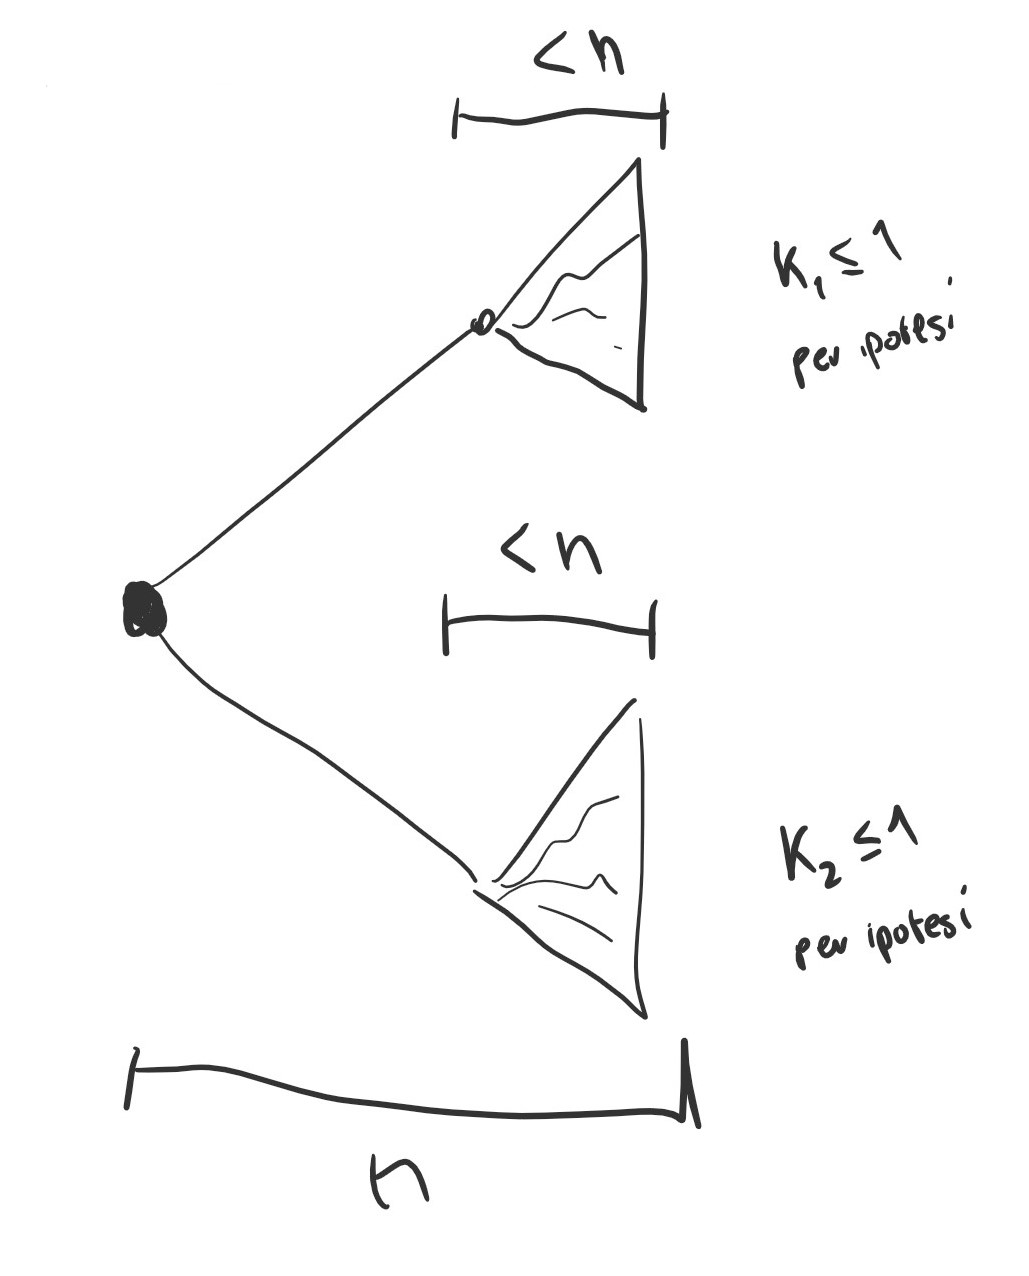
\includegraphics[width=0.45\linewidth]{immagini/img13}
\end{figure}


Quindi per ipotesi i due sottoalberi profondi al massimo $n-1$ hanno $K \leq 1$; supponendo di 'attaccarli' ad un nuovo nodo significa appendere come prefisso di tutte le codeword un altro simbolo.
\begin{figure}[h]
	\centering
	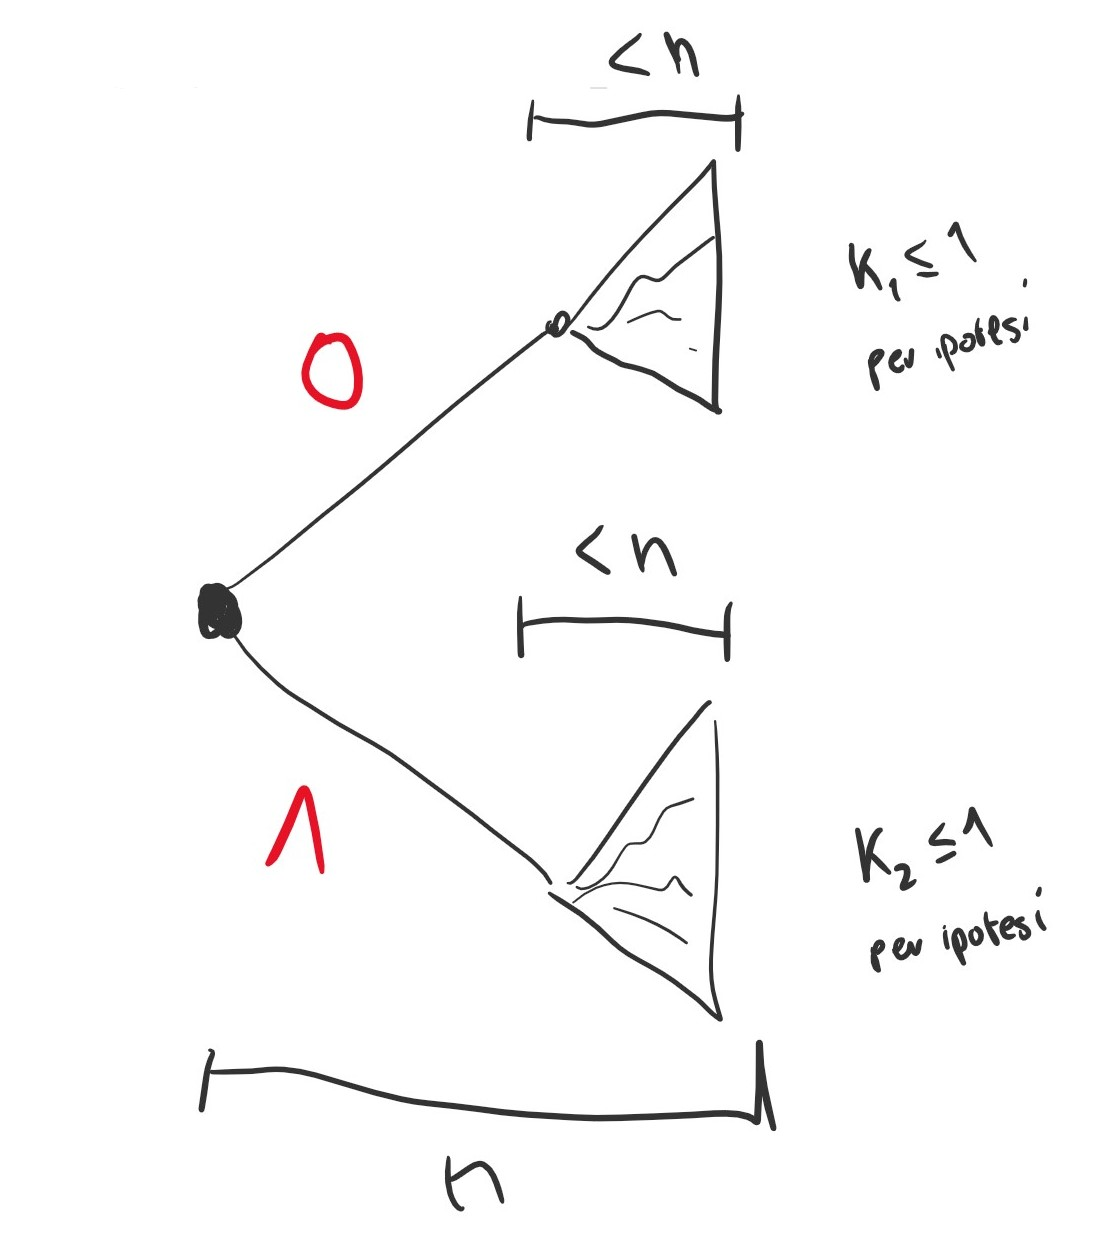
\includegraphics[width=0.45\linewidth]{immagini/img14}
\end{figure}

Come cambiano le $K$ quando allungo di uno le lunghezze delle codeword? Tutte le $\ell_i$ diventano $\ell_i + 1$:
\begin{equation*}
K_1 = \sum_{i=1}^{q}\frac{1}{r^{\ell_i+1}} = \sum_{i=1}^{q}(\frac{1}{r^{\ell_i}}\frac{1}{r}) = \frac{1}{r}\sum_{i=1}^{q}\frac{1}{r^{\ell_i}}
\end{equation*}

Quindi il contributo dato da ognuno dei due sottoalberi al calcolo di $K$ totale è dato da $\frac{1}{2}K_i$ (per $r=2$).
Il $K$ relativo all'albero totale quindi diventa:
\begin{equation*}
K = \frac{1}{2}K_1 + \frac{1}{2}K_2 = \frac{1}{2}(K_1 + K_2)
\end{equation*}
Sappiamo che $K_1 \leq 1$ e che $K_2 \leq 1$, quindi la loro somma sarà sicuramente $\leq 2$. La somma, moltiplicata per $\frac{1}{2}$ è $\leq 1$; quindi possiamo scrivere:
\begin{equation*}
K \leq 1
\end{equation*}
che è quello che volevamo dimostrare.\\

In caso $n$ non fosse $n=2$ bisogna solo creare più alberi di profondità 1 nel caso base:

\begin{figure}[H]
	\centering
	\vspace{4mm}
	\begin{tikzpicture}
	[
	grow                    = right,
	sibling distance        = 6em,
	level distance          = 7em,
	edge from parent/.style = {draw, -latex},
	every node/.style       = {font=\footnotesize},
	sloped
	]
	\node [root] {}
	child { node [dummy] {$s_m$}
		edge from parent node [below] {$m-1$}}
	child { node [dummy] {}
		edge from parent node [above] {...}}
	child { node [dummy] {$s_1$}
		edge from parent node [above] {0}};
	\end{tikzpicture}
\end{figure}

Dato che $m \leq r$ (delle $r$ foglie possibili ne ha solo $m$)

\begin{equation*}
K=m(\frac{1}{r}) = \frac{m}{r} \leq 1
\end{equation*}

Nel passo induttivo il numero di sottoalberi sarà $m$, e quando attacchiamo i sottoalberi alla nuova radice il nuovo $K$ verrà
\begin{equation*}
K=\frac{1}{r}K_1+\frac{1}{r}K_2+...+\frac{1}{r}K_m
\end{equation*}

\newpage

Dimostriamo ora la seconda parte, ovvero "$k\leq 1 \rightarrow$ esiste codice istantaneo $r$-ario per $q$ simboli e codeword di lunghezze $\ell_1,\ell_2,...,\ell_q$".

Partiamo dall'ipotesi che $K \leq 1$, successivamente definiamo $\ell$ come:
\begin{equation*}
\ell = max\{\ell_1, \ell_2,...,\ell_q\}
\end{equation*}
Inoltre chiamo $t_j$ il numero di codeword di lunghezza $j$.

Riscriviamo $K$ in questo modo:
\begin{equation*}
K = \sum_{i=1}^{q}\frac{1}{r^{\ell_i}} = \sum_{i=1}^{\ell}t_i\cdot\frac{1}{r^i}
\leq 1
\end{equation*}
Posso riscriverlo in questo modo perchè è come se stessi raccogliendo le codeword di lunghezza uguale $t_i$.
Moltiplico per $r^\ell$ entrambi i membri:
\begin{equation*}
\sum_{i=1}^{\ell}t_ir^{\ell-1} \leq r^\ell
\end{equation*}
Questo equivale a:
\begin{equation*}
	t_1r^{\ell-1}+t_2r^{\ell-2}+..+t_{\ell-1}r+t_\ell \leq r^\ell
\end{equation*}
Isolo $t_\ell$:
\begin{equation*}
t_\ell \leq r^{\ell} -t_1r^{\ell-1}-t_2r^{\ell-2}-...-t_{\ell-1}r
\end{equation*}
So che $t_\ell$ è maggiore o uguale a zero (numero di codeword di lunghezza $\ell$)
\begin{equation*}
0 \leq t_\ell \leq r^{\ell} -t_1r^{\ell-1}-t_2r^{\ell-2}-...-t_{\ell-1}r
\end{equation*}
Quindi ho posto un vincolo al numero massimo di codeword di lunghezza $\ell$. Ora considero solo questo pezzo:
\begin{equation*}
0 \leq r^{\ell} -t_1r^{\ell-1}-t_2r^{\ell-2}-...-t_{\ell-1}r
\end{equation*}
Divido tutto per $r$ e porto a sinistra l'ultimo termine $t_{\ell-1}r$:
\begin{equation*}
0 \leq t_{\ell-1} \leq r^{\ell-1} - t_1r^{\ell-2}-t_2r^{\ell-3}-...-t_{\ell-2}r
\end{equation*}
Posso rifarlo per tutti i $t$:
\begin{equation*}
0 \leq t_{\ell-2} \leq ...
\end{equation*}
E mi fermo a 
\begin{equation}
0 \leq t_2 \leq r^2-t_1r
\end{equation}
\begin{equation}
0 \leq t_1 \leq r \; \; \; \; \; \; \; \; \; \; \;
\end{equation}
Quindi sto ponendo dei limiti alle codeword di lunghezza 1, di lunghezza 2, ecc...

A questo punto, partendo dall'ultima equazione, risalgo.\\
Quante codeword di lunghezza 1 posso creare? (Equazione 44) Boh, di sicuro un numero compreso fra 0 e $r$.\\
Poi mi chiedo quante di lunghezza 2 (Equazione 43)? Boh quelle rimaste sono $r-t_1$, da queste posso appendere un carattere qualsiasi, quindi $r$.
Per cui ne posso creare al masssimo $r^2-t_1r$

Proseguendo in questo modo verifico tutte le disuguaglianze, partendo dalla sola ipotesi che $K \leq 1$

\medskip

Appunti "Disugliaglianza di Kraft MacMillan.pdf"
\end{dimostrazione}



